% LaTeX support: latex@mdpi.com
% For support, please attach all files needed for compiling as well as the log file, and specify your operating system, LaTeX version, and LaTeX editor.

%=================================================================
\documentclass[algorithms,article,submit,pdftex,oneauthors]{Definitions/mdpi}

%--------------------
% Class Options:
%--------------------
%----------
% journal
%----------
% Choose between the following MDPI journals:
% acoustics, actuators, addictions, admsci, adolescents, aerobiology, aerospace, agriculture, agriengineering, agrochemicals, agronomy, ai, air, algorithms, allergies, alloys, analytica, analytics, anatomia, animals, antibiotics, antibodies, antioxidants, applbiosci, appliedchem, appliedmath, applmech, applmicrobiol, applnano, applsci, aquacj, architecture, arm, arthropoda, arts, asc, asi, astronomy, atmosphere, atoms, audiolres, automation, axioms, bacteria, batteries, bdcc, behavsci, beverages, biochem, bioengineering, biologics, biology, biomass, biomechanics, biomed, biomedicines, biomedinformatics, biomimetics, biomolecules, biophysica, biosensors, biotech, birds, bloods, blsf, brainsci, breath, buildings, businesses, cancers, carbon, cardiogenetics, catalysts, cells, ceramics, challenges, chemengineering, chemistry, chemosensors, chemproc, children, chips, cimb, civileng, cleantechnol, climate, clinpract, clockssleep, cmd, coasts, coatings, colloids, colorants, commodities, compounds, computation, computers, condensedmatter, conservation, constrmater, cosmetics, covid, crops, cryptography, crystals, csmf, ctn, curroncol, cyber, dairy, data, ddc, dentistry, dermato, dermatopathology, designs, devices, diabetology, diagnostics, dietetics, digital, disabilities, diseases, diversity, dna, drones, dynamics, earth, ebj, ecologies, econometrics, economies, education, ejihpe, electricity, electrochem, electronicmat, electronics, encyclopedia, endocrines, energies, eng, engproc, entomology, entropy, environments, environsciproc, epidemiologia, epigenomes, est, fermentation, fibers, fintech, fire, fishes, fluids, foods, forecasting, forensicsci, forests, foundations, fractalfract, fuels, future, futureinternet, futurepharmacol, futurephys, futuretransp, galaxies, games, gases, gastroent, gastrointestdisord, gels, genealogy, genes, geographies, geohazards, geomatics, geosciences, geotechnics, geriatrics, grasses, gucdd, hazardousmatters, healthcare, hearts, hemato, hematolrep, heritage, higheredu, highthroughput, histories, horticulturae, hospitals, humanities, humans, hydrobiology, hydrogen, hydrology, hygiene, idr, ijerph, ijfs, ijgi, ijms, ijns, ijpb, ijtm, ijtpp, ime, immuno, informatics, information, infrastructures, inorganics, insects, instruments, inventions, iot, j, jal, jcdd, jcm, jcp, jcs, jcto, jdb, jeta, jfb, jfmk, jimaging, jintelligence, jlpea, jmmp, jmp, jmse, jne, jnt, jof, joitmc, jor, journalmedia, jox, jpm, jrfm, jsan, jtaer, jvd, jzbg, kidneydial, kinasesphosphatases, knowledge, land, languages, laws, life, liquids, literature, livers, logics, logistics, lubricants, lymphatics, machines, macromol, magnetism, magnetochemistry, make, marinedrugs, materials, materproc, mathematics, mca, measurements, medicina, medicines, medsci, membranes, merits, metabolites, metals, meteorology, methane, metrology, micro, microarrays, microbiolres, micromachines, microorganisms, microplastics, minerals, mining, modelling, molbank, molecules, mps, msf, mti, muscles, nanoenergyadv, nanomanufacturing,\gdef\@continuouspages{yes}} nanomaterials, ncrna, ndt, network, neuroglia, neurolint, neurosci, nitrogen, notspecified, %%nri, nursrep, nutraceuticals, nutrients, obesities, oceans, ohbm, onco, %oncopathology, optics, oral, organics, organoids, osteology, oxygen, parasites, parasitologia, particles, pathogens, pathophysiology, pediatrrep, pharmaceuticals, pharmaceutics, pharmacoepidemiology,\gdef\@ISSN{2813-0618}\gdef\@continuous pharmacy, philosophies, photochem, photonics, phycology, physchem, physics, physiologia, plants, plasma, platforms, pollutants, polymers, polysaccharides, poultry, powders, preprints, proceedings, processes, prosthesis, proteomes, psf, psych, psychiatryint, psychoactives, publications, quantumrep, quaternary, qubs, radiation, reactions, receptors, recycling, regeneration, religions, remotesensing, reports, reprodmed, resources, rheumato, risks, robotics, ruminants, safety, sci, scipharm, sclerosis, seeds, sensors, separations, sexes, signals, sinusitis, skins, smartcities, sna, societies, socsci, software, soilsystems, solar, solids, spectroscj, sports, standards, stats, std, stresses, surfaces, surgeries, suschem, sustainability, symmetry, synbio, systems, targets, taxonomy, technologies, telecom, test, textiles, thalassrep, thermo, tomography, tourismhosp, toxics, toxins, transplantology, transportation, traumacare, traumas, tropicalmed, universe, urbansci, uro, vaccines, vehicles, venereology, vetsci, vibration, virtualworlds, viruses, vision, waste, water, wem, wevj, wind, women, world, youth, zoonoticdis
% For posting an early version of this manuscript as a preprint, you may use "preprints" as the journal. Changing "submit" to "accept" before posting will remove line numbers.

%---------
% article
%---------
% The default type of manuscript is "article", but can be replaced by:
% abstract, addendum, article, book, bookreview, briefreport, casereport, comment, commentary, communication, conferenceproceedings, correction, conferencereport, entry, expressionofconcern, extendedabstract, datadescriptor, editorial, essay, erratum, hypothesis, interestingimage, obituary, opinion, projectreport, reply, retraction, review, perspective, protocol, shortnote, studyprotocol, systematicreview, supfile, technicalnote, viewpoint, guidelines, registeredreport, tutorial
% supfile = supplementary materials

%----------
% submit
%----------
% The class option "submit" will be changed to "accept" by the Editorial Office when the paper is accepted. This will only make changes to the frontpage (e.g., the logo of the journal will get visible), the headings, and the copyright information. Also, line numbering will be removed. Journal info and pagination for accepted papers will also be assigned by the Editorial Office.

%------------------
% moreauthors
%------------------
% If there is only one author the class option oneauthor should be used. Otherwise use the class option moreauthors.

%---------
% pdftex
%---------
% The option pdftex is for use with pdfLaTeX. Remove "pdftex" for (1) compiling with LaTeX & dvi2pdf (if eps figures are used) or for (2) compiling with XeLaTeX.

%=================================================================
% MDPI internal commands - do not modify
\firstpage{1}
\makeatletter
\setcounter{page}{\@firstpage}
\makeatother
\pubvolume{1}
\issuenum{1}
\articlenumber{0}
\pubyear{2023}
\copyrightyear{2023}
%\externaleditor{Academic Editor: Firstname Lastname}
\datereceived{ }
\daterevised{ } % Comment out if no revised date
\dateaccepted{ }
\datepublished{ }
%\datecorrected{} % For corrected papers: "Corrected: XXX" date in the original paper.
%\dateretracted{} % For corrected papers: "Retracted: XXX" date in the original paper.
\hreflink{https://doi.org/} % If needed use \linebreak
%\doinum{}
%\pdfoutput=1 % Uncommented for upload to arXiv.org

%=================================================================
% Add packages and commands here. The following packages are loaded in our class file: fontenc, inputenc, calc, indentfirst, fancyhdr, graphicx, epstopdf, lastpage, ifthen, float, amsmath, amssymb, lineno, setspace, enumitem, mathpazo, booktabs, titlesec, etoolbox, tabto, xcolor, colortbl, soul, multirow, microtype, tikz, totcount, changepage, attrib, upgreek, array, tabularx, pbox, ragged2e, tocloft, marginnote, marginfix, enotez, amsthm, natbib, hyperref, cleveref, scrextend, url, geometry, newfloat, caption, draftwatermark, seqsplit
% cleveref: load \crefname definitions after \begin{document}

\usepackage{gensymb}
\usepackage{accents}
\usepackage{xspace}

%Definition des mises en page
\definecolor{gray75}{gray}{0.75}
\definecolor{gray95}{gray}{0.95}
\definecolor{gray50}{gray}{0.50}
\definecolor{gray40}{gray}{0.40}
\definecolor{redcolor}{rgb}{0.6,0.0,0.0}
\definecolor{greencolor}{rgb}{0.0,0.6,0.0}  % Green color

% Definition des listings avec langage par défaut Python
\usepackage{listings}

%\lstnewenvironment{CppListing}[1][]
%    {\lstset{language=C++,
%        #1}%
%        \noindent\begin{minipage}{\textwidth}\csname\@lst @SetFirstNumber\endcsname\end{minipage}}
%        {\csname\@lst @SaveFirstNumber\endcsname}

\lstnewenvironment{FortranListing}[1][]
    {\lstset{language=[77]Fortran,#1}}{}

\lstnewenvironment{PythonListing}[1][]
    {\lstset{language=Python,morekeywords={as,assert,with,yield},#1}}{}


\lstset{language=Python,
keywordstyle=\color{redcolor},
numberstyle=\footnotesize\color{gray40},
numbers=left,
%frame=single,xleftmargin=5.0ex,xrightmargin=1.0ex,
literate={-} {\textrm{-}}{1},
showstringspaces=false,
commentstyle=\color{gray50},
stringstyle=\color{greencolor},
basicstyle=\sffamily\small\upshape,
%escapeinside={<@}{@>},
backgroundcolor=\color{gray95},
%breaklines=true,
%postbreak=\usebox\mypostbreak,
%rulecolor=\color{gray50}
}

\usepackage[labelformat=simple]{subcaption}
\renewcommand\thesubfigure{\alph{subfigure}}
\DeclareCaptionLabelFormat{subcaptionlabel}{\normalfont(\textbf{#2}\normalfont)}
\captionsetup[subfigure]{labelformat=subcaptionlabel}

\DeclareRobustCommand{\w}{\mbox{\large\ensuremath{\mathsf{w}}}}
\DeclareRobustCommand{\dotp}{\boldsymbol{\cdot}}
\DeclareRobustCommand{\e}[1]{{\rm e}^{#1}}
%\DeclareRobustCommand{\lay}[1]{^{(#1)}}
\DeclareRobustCommand{\lay}[1]{_{[#1]}}
\DeclareRobustCommand{\Lay}[1]{\mbox{$[#1]$}}
\DeclareRobustCommand{\mdot}[1]{\accentset{\mbox{\bfseries .}}{#1}}
\DeclareRobustCommand{\ie}{i.e.,\@\xspace}
\DeclareRobustCommand{\eal}{et \emph{al.}\@\xspace}
\DeclareRobustCommand{\eg}{e.g.,\@\xspace}
\DeclareRobustCommand{\MSE}{\text{E}_\text{MS}}
\DeclareRobustCommand{\RMSE}{\text{E}_\text{RMS}}
\DeclareRobustCommand{\MARE}{\text{E}_\text{MAR}}
\DeclareRobustCommand{\R}{\text{R}}
\DeclareRobustCommand{\ps}{\text{s}^{-1}}
\DeclareRobustCommand{\mr}[2]{\multirow{#1}{*}{#2}}
\DeclareRobustCommand{\MPa}{\text{MPa}}
\DeclareRobustCommand{\GPa}{\text{GPa}}
\DeclareRobustCommand{\Sig}{\mbox{\large\ensuremath{\boldsymbol{\sigma}}}}
\DeclareRobustCommand{\Eps}{\mbox{\large\ensuremath{\boldsymbol{\varepsilon}}}}
\DeclareRobustCommand{\var}[1]{\textsf{#1}}

% This is used to add comments into the text
%
% Will have to be removed from final version
%
\usepackage{soul}
\usepackage{color}
\definecolor{VWyellow}{RGB}{255,251,150}
\DeclareRobustCommand{\OP}[1]{\begingroup\sethlcolor{VWyellow}\textcolor{red}{\hl{\textbf{O.P.:} #1}}\endgroup}
\DeclareRobustCommand{\OPP}[1]{\begingroup\sethlcolor{VWyellow}\textcolor{red}{\hl{\textbf{O.P.:} In previous sentence #1}}\endgroup}

%=================================================================
% Please use the following mathematics environments: Theorem, Lemma, Corollary, Proposition, Characterization, Property, Problem, Example, ExamplesandDefinitions, Hypothesis, Remark, Definition, Notation, Assumption
%% For proofs, please use the proof environment (the amsthm package is loaded by the MDPI class).

%=================================================================
% Full title of the paper (Capitalized)
\Title{Title}

% MDPI internal command: Title for citation in the left column
\TitleCitation{Title}

% Author Orchid ID: enter ID or remove command
\newcommand{\orcidauthorA}{0000-0001-7367-5453} % Add \orcidA{} behind the author's name
%\newcommand{\orcidauthorB}{0000-0000-0000-000X} % Add \orcidB{} behind the author's name

% Authors, for the paper (add full first names)
\Author{Olivier Pantal\'{e}\orcidA{}}

%\longauthorlist{yes}

% MDPI internal command: Authors, for metadata in PDF
\AuthorNames{Olivier Pantal\'{e}}

% MDPI internal command: Authors, for citation in the left column
\AuthorCitation{Pantal\'{e}, O.}
% If this is a Chicago style journal: Lastname, Firstname, Firstname Lastname, and Firstname Lastname.

% Affiliations / Addresses (Add [XX] after \address if there is only one affiliation.)
\address[1]{Laboratoire Génie de Production, Institut National Polytechnique/Ecole Nationale d'Ingénieurs de Tarbes, Université de Toulouse, 47 Av d'Azereix, F-65016 Tarbes, France; Olivier.Pantale@enit.fr; Tel.: +33-562442933}

% Current address and/or shared authorship
%\firstnote{Current address: Affiliation 3.}
%\secondnote{These authors contributed equally to this work.}
% The commands \thirdnote{} till \eighthnote{} are available for further notes

%\simplesumm{} % Simple summary

%\conference{} % An extended version of a conference paper

% Abstract (Do not insert blank lines, i.e. \\)
\abstract{A single paragraph of about 200 words maximum. For research articles, abstracts should give a pertinent overview of the work. We strongly encourage authors to use the following style of structured abstracts, but without headings: (1) Background: place the question addressed in a broad context and highlight the purpose of the study; (2) Methods: describe briefly the main methods or treatments applied; (3) Results: summarize the article's main findings; (4) Conclusions: indicate the main conclusions or interpretations. The abstract should be an objective representation of the article, it must not contain results which are not presented and substantiated in the main text and should not exaggerate the main conclusions.}

% Keywords
\keyword{ANN flow law; Constitutive Behavior; Numerical Implementation; VUHARD ; Activation Functions; Abaqus Explicit}

% The fields PACS, MSC, and JEL may be left empty or commented out if not applicable
%\PACS{J0101}
%\MSC{}
%\JEL{}

%%%%%%%%%%%%%%%%%%%%%%%%%%%%%%%%%%%%%%%%%%
% Only for the journal Diversity
%\LSID{\url{http://}}

%%%%%%%%%%%%%%%%%%%%%%%%%%%%%%%%%%%%%%%%%%
% Only for the journal Applied Sciences
%\featuredapplication{Authors are encouraged to provide a concise description of the specific application or a potential application of the work. This section is not mandatory.}
%%%%%%%%%%%%%%%%%%%%%%%%%%%%%%%%%%%%%%%%%%

%%%%%%%%%%%%%%%%%%%%%%%%%%%%%%%%%%%%%%%%%%
% Only for the journal Data
%\dataset{DOI number or link to the deposited data set if the data set is published separately. If the data set shall be published as a supplement to this paper, this field will be filled by the journal editors. In this case, please submit the data set as a supplement.}
%\datasetlicense{License under which the data set is made available (CC0, CC-BY, CC-BY-SA, CC-BY-NC, etc.)}

%%%%%%%%%%%%%%%%%%%%%%%%%%%%%%%%%%%%%%%%%%
% Only for the journal Toxins
%\keycontribution{The breakthroughs or highlights of the manuscript. Authors can write one or two sentences to describe the most important part of the paper.}

%%%%%%%%%%%%%%%%%%%%%%%%%%%%%%%%%%%%%%%%%%
% Only for the journal Encyclopedia
%\encyclopediadef{For entry manuscripts only: please provide a brief overview of the entry title instead of an abstract.}

%%%%%%%%%%%%%%%%%%%%%%%%%%%%%%%%%%%%%%%%%%
% Only for the journal Advances in Respiratory Medicine
%\addhighlights{yes}
%\renewcommand{\addhighlights}{%

%\noindent This is an obligatory section in “Advances in Respiratory Medicine”, whose goal is to increase the discoverability and readability of the article via search engines and other scholars. Highlights should not be a copy of the abstract, but a simple text allowing the reader to quickly and simplified find out what the article is about and what can be cited from it. Each of these parts should be devoted up to 2~bullet points.\vspace{3pt}\\
%\textbf{What are the main findings?}
% \begin{itemize}[labelsep=2.5mm,topsep=-3pt]
% \item First bullet.
% \item Second bullet.
% \end{itemize}\vspace{3pt}
%\textbf{What is the implication of the main finding?}
% \begin{itemize}[labelsep=2.5mm,topsep=-3pt]
% \item First bullet.
% \item Second bullet.
% \end{itemize}
%}

%%%%%%%%%%%%%%%%%%%%%%%%%%%%%%%%%%%%%%%%%%
\begin{document}

%----------------------------------------------------------------------------------
\section{Introduction}\label{sec:Introduction}
%----------------------------------------------------------------------------------

In industry and research, numerical simulations of the behavior of structures subjected to severe thermomechanical loadings, such as in the case of high-temperature forming of metallic materials, are typically based on the use of commercial finite element (FE) codes, such as Abaqus~\cite{Abaqus}, or academic codes.
The results of these numerical simulations are strongly dependent on the constitutive equations and the identification of their parameters from experimental tests, which form the basis of the description of the thermomechanical behavior of materials.
The quality and accuracy of the results of any numerical simulation depend on the choice of these behavior laws (thus their mathematical formulation) and the user's ability to identify the coefficients of these behavior laws for a given material by conducting experiments under conditions similar to those encountered during the actual loading of the structure in service that one wishes to design.
Depending on the nature of the thermomechanical loadings involved, whether quasi-static, dynamic, at high or low temperatures, these tests are based on quasi-static or dynamic tensile or compression tests, tests on thermomechanical simulators such as Gleeble~\cite{Lin-2009-MFS, Kumar-2016-TMS, Yu-2019-RCR}, or impact tests using gas guns or Hopkinson bars~\cite{Kolsky-1949-IMP}.

\subsection{Constitutive behavior and material flow law}\label{subsec:ConstBehavior}

Thermomechanical behavior laws within numerical integration algorithms~\cite{Ponthot-2002-USU} make use of flow law functions which, due to the nature of the materials and the phenomena involved (work hardening, dislocation movement, structural hardening, phase transformations, etc.), are highly non-linear.
The validity of these flow laws is limited to a certain range of deformations, strain rates and temperatures.
For the implementation of a thermomechanical simulation of a forming process, the behavior laws define the dependence of the material's flow stress on three input variables: the strain, the strain rate, and the temperature, so that the general form of the flow law can be expressed with the following equation:
\begin{equation}
\sigma = f\left(\varepsilon, \mdot{\varepsilon}, T\right),\label{eq:GenFlow}
\end{equation}
where~$\sigma$ is the flow stress of the material, $\varepsilon$ is the strain, $\mdot{\varepsilon}$ is the strain rate, $T$ is the temperature and~$f()$ represents the flow law that expresses the non-linear relationship between the stress and the thermomechanical variables ($\varepsilon$, $\mdot{\varepsilon}$ and~$T$).

Historically, the first mathematical formulations for the simulation of hot forming processes appeared in the 1950s.
The flow laws used were essentially power laws, describing the relationship between stress and strain.
These laws were later adapted to take into account the effect of temperature.
From the 1970s, thermomechanical models evolved to include time dependence.
This means that thermomechanical flow laws became dependent on strain rate and time.
The Johnson--Cook flow law~\cite{Johnson-1983-CMD}, the Zerilli--Armstrong~\cite{Zerilli-1987-DMB} and the Arrhenius flow law~\cite{Jonas-1969}, which are commonly used in the simulation of forming processes, were developed at this time.
Subsequently, researchers began to focus on modeling the effects of plastic flow in high-temperature metals and improving previous models to overcome some of their limitations.
This led to the development of modified versions of previous models, notably the Johnson--Cook model~\cite{Duc-Toan-2012-MJC, Li-2013-MJC, Zhang-2015}, the Zerilli--Armstrong model~\cite{He-2014-MZA, Gurusamy-2017-OTP, Yu-2020-FSM} and the Arrhenius model~\cite{Zhan-2014-CMF, Liang-2022}, as well as comparative studies of the respective abilities of these models to cope with increasingly complex thermomechanical behavior~\cite{Liu-2020-FSP}.
Of all these models, the Johnson--Cook model is generally the most widely used because it is the simplest to identify and use, requiring the determination of just 5 parameters~\cite{Zeng-2022-TCR}.
Nevertheless, a large number of works in the literature point to the shortcomings of flow law models such as Johnson--Cook's when numerical simulations require a high degree of correlation with experiment and when thermomechanical conditions become severe.

Whatever the choice made regarding the formulation of the flow law to be used, it is imperative, based on experimental tests conducted in laboratory settings under conditions closely resembling real-world applications, to identify the parameters of these flow laws by methods typically grounded in approaches for minimizing the experimental/simulated discrepancy.
The primary challenge confronting researchers, once the experimental behavior characterization tests have been carried out, concerns the actual selection of the flow law to use, based on the observations made on these test results.
This selection is greatly influenced by the availability of these flow laws within the finite element analysis software employed.
For example, a user of the Abaqus FE code is more inclined to opt for a Johnson--Cook flow law, since it is natively implemented.
The choice of an alternative form of flow law, such as Zerilli--Armstrong or Arrhenius, necessitates, in the case of employing the Abaqus software, that the user personally undertake the computation of material yield stress~$\sigma$ through a VUMAT subroutine in Fortran, as proposed by Gao \eal~\cite{Gao-2007-FRT}, Ming \eal~\cite{Ming-2018-ERV} for a Johnson-Cook flow law, or Liang \eal~\cite{Liang-2022} for an Arrhenius-type flow law.
This process is time-consuming, demands a certain level of expertise, and requires knowledge concerning flow law formulations, numerical integration, Fortran programming, as well as the development and testing of models.

The development and numerical implementation of a user behavior law on the Abaqus code requires the calculation of the flow stress~$\sigma$ as defined by Equation (\ref{eq:GenFlow}) and the three derivatives of this flow stress with respect to strain~$\varepsilon$, strain rate~$\mdot{\varepsilon}$ and temperature~$T$.
This evaluation can quickly become relatively complex and time-consuming as the complexity of the flow law increases.
The choice of a flow law formulation to be used for the simulation of a thermomechanical forming problem is therefore guided by two distinct and complementary aspects: on the one hand by the material behavior and the consideration of process physics, but above all by the availability of this flow law in the FE calculation code used for the simulation.
The choice of flow law to be used is mainly guided by the list of flow laws available in the finite element code used, and very often this choice is made to the detriment of model quality.

As an example, Tize Mha \eal~\cite{Tize-2023-IEP}, identified several flow laws from experimental compression tests carried out on a Gleeble-3800 thermomechanical simulator for a P20 medium-carbon steel intended for the production of foundry molds.
The work considered several flow laws and their identification from the results of these tests, including Johnson--Cook, Modified Zerilli--Armstrong, Arrhenius, Hensel--Spittle and PTM.
The results showed that over the range of strain rates and temperatures tested, only the Arrhenius flow law was capable of reproducing the compression behavior of this material with a fidelity compatible with industrial applications.

Based on all these considerations, we have recently proposed in Pantalé \eal~\cite{Pantale-2021-EIN, Pantale-2023-DIA} a new approach for the formulation of flow laws based on the ability of artificial neural networks (ANNs) to behave as universal approximators as reported by Minsky \eal~\cite{Minsky-1969-PIC} and Hornik \eal~\cite{Hornik-1989-MFN}.
With this new approach, it is no longer necessary a priori to postulate a mathematical form of the constitutive equation for use in a finite element simulation.

Artificial neural networks have been the subject of extensive research in the field of thermomechanical plasticity modelingas reported by Gorji \eal~\cite{Gorji-2020} or Jamli \eal~\cite{Jamli-2019-SNN}.
These studies have delved into the utilization of ANNs for finite element analysis of metal forming processes and their application in characterizing meta-materials.
Lin \eal~\cite{Lin-2008} applied an ANN to predict the yield stress of 42CrMo4 steel in hot compression tests, revealing a strong correlation between experimental findings and model predictions.
ANNs have been successfully applied to predict the flow stress behavior of materials under hot working conditions~\cite{Stoffel-2018-ANN, Stoffel-2019-NNB}.
They have also been applied recently in micromechanics for polycrystalline metals by Ali \eal~\cite{Ali-2019-AAN}.
The domain of application has been extended to dynamic recrystallization of metal alloys by Wang \eal~\cite{Wang-2021-ANN}.
Some approaches mix analytical and ANN flow laws such as for example the work proposed by Cheng \eal~\cite{Cheng-2022-CWD} where the authors use a combination of an ANN with the Arrhenius equation to model the behavior of a GH4169 superalloy.
ANN behavior laws can also include chemical composition of materials in their formulation to increase the performance during simulation hot deformation for high-Mn steels with different concentrations as proposed by Churyumov \eal~\cite{Churyumov-2023-PTS}.

In the majority of the works presented in the previous paragraph, the authors work either on the proposal of a neural network model and its identification in relation to experimental tests, or on the use of a neural network within the framework of a numerical simulation of a process.
The approach proposed here is more complete in that we identify a neural network from experimental tests (in our case, cylinder compression tests on a Gleeble thermomechanical simulator), then identify the network parameters.
We then implement this network in the Abaqus FE code in the form of a user subroutine in Fortran, and subsequently validate and use this network in numerical simulations.
We therefore work on the entire calculation chain, from experimental data acquisition, through network formulation and learning, to implementation and use.

\subsection{Experimental tests and data}\label{subsec:ExpTests}

The material used for this study is a medium-carbon steel, type P20.
The experimental tests used for this work are identical to those previously published by Tize Mha \eal~\cite{Tize-2023-IEP} and concern hot compression tests, on a Gleeble-3800 thermomechanical simulator, of P20 steel cylinders with an initial diameter of~$d=10$~mm and a height of~$h_0=15$~mm.
Only the most relevant information about those experiments is reported here after.
In order to have a more complete knowledge about the compression tests conducted during this study, the interested reader can refer to Tize Mha \eal~\cite{Tize-2023-IEP}.
The imposed displacement was set to~$d=9$~mm, resulting in a reduction of~$60\%$ of the initial height.
Hot compression tests were performed for five temperature levels, namely~$1050~\celsius$, $1100~\celsius$, $1150~\celsius$, $1200~\celsius$, and~$1250~\celsius$, with the six strain rates of~$0.001~\ps$, $0.01~\ps$, $0.1~\ps$, $1~\ps$, $2.0~\ps$, and~$5~\ps$.
Figure \ref{fig:RawData} reports a plot of all 30 stress/strain curves extracted from the compression tests experiments.
\begin{figure}[h]
\centering
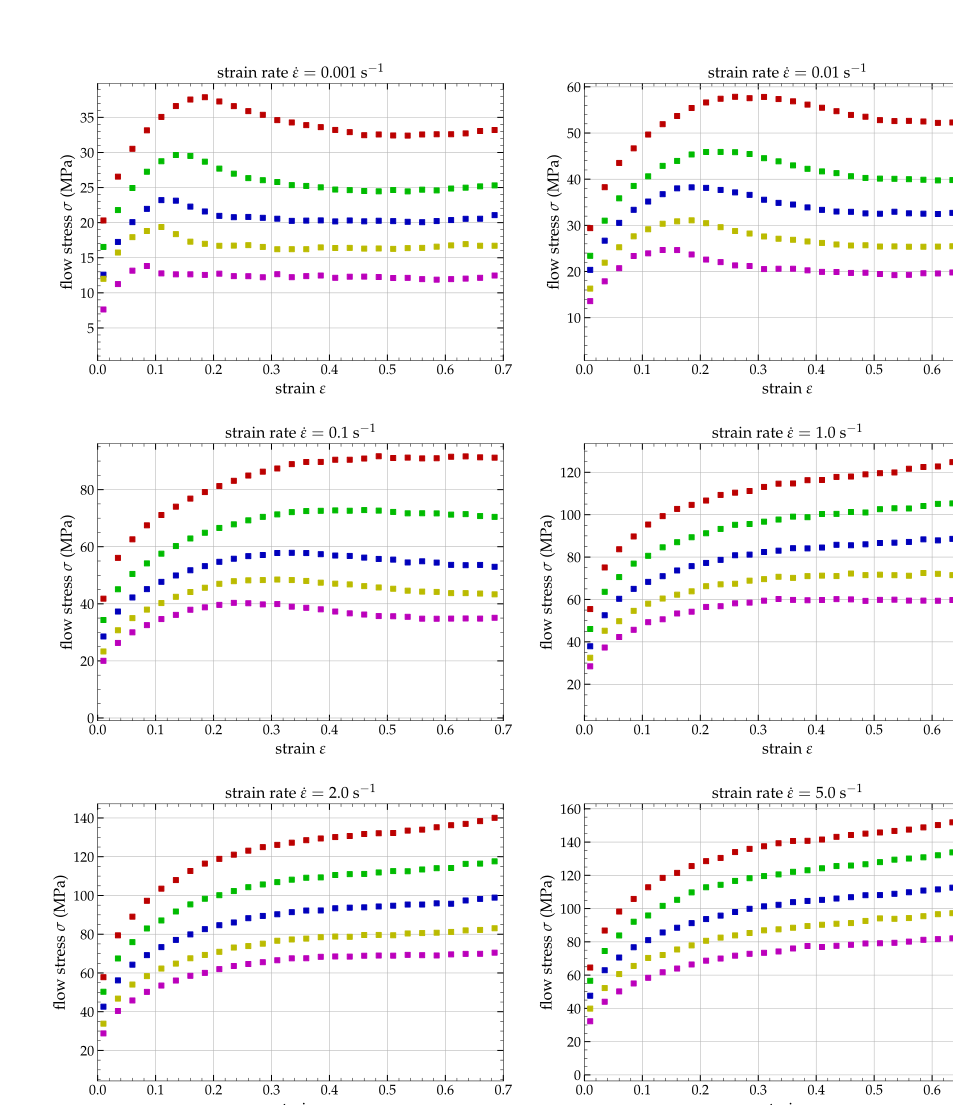
\includegraphics[width=0.9\columnwidth]{Figures/3Cr2Mo-raw}
\caption{Stress/strain curves of P20 alloy extracted from the Gleeble device for the five temperatures ($T$) and six strain rates ($\mdot{\varepsilon}$).}
\label{fig:RawData}
\end{figure}
The experimental database is composed of all strain/stress data for all 30 couples of strain rate and temperature.
Each strain/stress curve is composed of 701 equidistant strain values from~$\varepsilon=0.0$ to~$\varepsilon=0.7$ in~$\Delta\varepsilon=0.001$ increments.
The complete database is therefore composed of~$21~030$ quadruplets ($\varepsilon$, $\mdot{\varepsilon}$, $T$ and~$\sigma$).
This dataset will be used in the next Section to identify the ANN flow law parameters depending on the selected hyperparameters of the networks.

Section \ref{sec:ANN} is dedicated to the presentation of the material flow law based on an artificial neural network.
The first part is dedicated to a reminder of the basic notions on ANNs, with a section on the choice of activation functions to be used in the formulation.
The architecture chosen for the formulation of the flow laws based on a two-hidden-layer network will then be presented, together with the formulation of the derivatives of the output as a function of the input variables.
The learning methodology and the results in terms of network performance as a function of the activation functions selected will then be presented.
Section \ref{sec:Numerical} is dedicated to the numerical simulation of a compression test on the Abaqus computational code, integrating the ANN implemented as a user routine in Fortran.
The quality of the numerical solution obtained and its performance in terms of computational cost will be analyzed as a function of the network structure.
Finally, conclusions and future prospects are presented in the last section.

%----------------------------------------------------------------------------------
\section{Artificial Neural Network flow law}\label{sec:ANN}
%----------------------------------------------------------------------------------

As already proposed in Pantalé \eal~\cite{Pantale-2021-EIN, Pantale-2023-DIA}, the approach used here is to implement the constitutive flow law defined by a trained ANN as a Fortran subroutine into the Abaqus finite element code.
The ANN is trained on the basis of the Gleeble experiments as already introduced in Section \ref{sec:Introduction} and is used to compute the value of the flow stress~$\sigma$ as a function of the strain~$\varepsilon$, the strain rate~$\mdot{\varepsilon}$ and the temperature~$T$.
After the training phase, the weights and biases of the ANN are transcoded into a Fortran subroutine wich is compiled and linked with the libraries of the Abaqus FE code to include the thermomechanical behavior and compute the flow tress and its three derivatives~$\partial\sigma/\partial\varepsilon$, $\partial\sigma/\partial\mdot{\varepsilon}$ and~$\partial\sigma/\partial T$ needed by the radial-return algorithm of the FE code.

\subsection{ANN governing equations}\label{subsec:ANN-eqn}

\subsubsection{Network architecture}\label{subsubsec:ANN-arch}
According to Figure \ref{fig:ANN-2HL}, the ANN used for computing the flow stress~$\sigma$ from the strain~$\varepsilon$, the strain rate~$\mdot{\varepsilon}$ and the temperature~$T$ is a two hidden layers network as already proposed by Pantalé \eal~\cite{Pantale-2021-EIN, Pantale-2023-DIA}.
\begin{figure}[h]
\centering
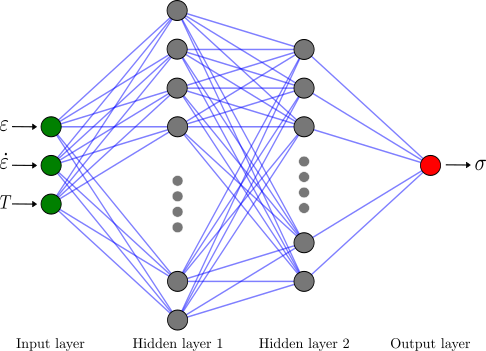
\includegraphics[width=0.55\columnwidth]{Figures/ANN-2HL}
\caption{Two hidden layers ANN architecture with 3 inputs neurons ($\varepsilon$, $\mdot{\varepsilon}$ and~$T$) and 1 output neuron ($\sigma$).}
\label{fig:ANN-2HL}
\end{figure}
The input of the neural network is a three component vector noted~$\overrightarrow{x}$.
Any hidden layer~\Lay{k}, containing~$n$ neurons, takes a weighted sum of the outputs~$\overrightarrow{\hat{y}}\lay{k-1}$ of the previous layer~\Lay{k-1}, containing~$m$ neurons, given by the following equation:
\begin{equation}
\overrightarrow{y}\lay{k} = \w\lay{k} \cdot \overrightarrow{\hat{y}}\lay{k-1}+ \overrightarrow{b}\lay{k}\label{eq:ANN-y},
\end{equation}
where~$\overrightarrow{y}\lay{k}$ contains the internal values of the neurons from summation at the layer level~\Lay{k}, $\w\lay{k}$ is the weight parameter matrix~$[n\times m]$ between layer~\Lay{k} and layer~\Lay{k-1}, $\overrightarrow{b}\lay{k}$ is the bias vector of the layer~\Lay{k} and~$\overrightarrow{\hat{y}}\lay{k-1}$ is the output vector of the layer~\Lay{k-1} after the application of the activation function defined here-after.
The total number of learning parameters~$N$ for any hidden layer~\Lay{k} is the sum of the number of weights and the number of biases in the layer~\Lay{k}, i.e. $N=n(m+1)$.
After the summation operation defined by equation (\ref{eq:ANN-y}), each hidden layer~\Lay{k} provides an output vector~$\overrightarrow{\hat{y}\lay{k}}$ calculated from an activation function~$f\lay{k}$ according to the following equation:
\begin{equation}
\overrightarrow{\hat{y}}\lay{k}=f\lay{k}(\overrightarrow{y}\lay{k}).
\label{eq:ANN-f}
\end{equation}
This process is repeated for each hidden layer of the neural network until we reach the output layer where the formulation differ, so that the output~$s$ of the neural network is given by:
\begin{equation}
s = \overrightarrow{w}^T \dotp \overrightarrow{\hat{y}}\lay{2} + b\label{eq:ANN-s},
\end{equation}
where~$\overrightarrow{w}$ is the vector of the output weights of the ANN and~$b$ is the bias associated to the output neuron.
As usually done in a regression approach, there is no activation function associated to the output neuron of the network (or some authors consider here a linear activation function).

\subsubsection{Activation functions}\label{subsubsec:ANN-act}

At the heart of ANNs lies the concept of activation functions, pivotal elements that determine how information is transformed within the network's neurons.
The choice of activation functions is a critical design decision, as these functions greatly influence the network's capacity to learn and represent complex patterns in data.
The selection of activation functions is guided by their distinct properties, including non-linearity, differentiability, and computational efficiency.

%An activation function is a function that acts on the output of all neurons of the hidden layers and helps the ANN to learn complex non-linear features of the data to process.
In regression ANNs, the choice of activation functions is typically driven by the need to approximate continuous output values rather than class labels.
Many studies have been proposed concerning the right activation function to use depending on the physical problem to solve such as the review proposed by Dubey \eal~\cite{Dubey-2022-AFD} or Jagtap \eal~\cite{Jagtap-2023-HIA}.
The key aspect of the activation function is its capacity to introduce non-linearity into the network to capture non-linear features.
Without this non-linearity, the neural network behaves like a linear regression model.
According to and Hornik \eal~\cite{Hornik-1989-MFN}, the activation function must be bounded, non-constant, monotonically increasing, and continuous to ensure the universal approximation property of the neural network.
A number of activations functions can be used in neural networks.

In a previous published work~\cite{Pantale-2021-EIN, Pantale-2023-DIA}, we have mostly used the Sigmoid activation function for the ANN flow laws.
In the present paper, we are going to explore other activations functions and their influence on the final results, up-to the implementation into a finite element code such as the Abaqus software.
Among the number of activations functions available in the literature, we have selected the six ones reported in Figure \ref{fig:ActFunctions}.
\begin{figure}[h]
\centering
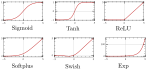
\includegraphics[width=0.8\columnwidth]{Figures/ActFunctions}
\caption{Activation functions used in ANNs.}
\label{fig:ActFunctions}
\end{figure}

The Sigmoid activation function~\cite{Han-1995-ISF}, also known as the logistic activation function, is a widely used activation function in ANNs.
It was originally developed in the field of logistic regression and later adapted for use in neural networks.
It maps any input to an output in the range~$[0,1]$, making it suitable for tasks where the network's output needs to represent probabilities or values between 0 and 1.
The Sigmoid activation function~$f(x)$ and its derivative~$f'(x)$ are defined by the following equations:
\begin{equation}
f(x) = \frac{1}{1+\e{-x}}\qquad \text{and}\qquad f'(x) = f(x)\left(1-f(x)\right).\label{eq:act-sig}
\end{equation}
This activation function has been widely used until the early 1990s.
Its main advantage is that it is bounded, while its main drawbacks are the vanishing gradient problem, an output not centered on zero and saturation for large input values.

From 1990s to 2000s, the hyperbolic tangent activation function has been introduced and was preferred for the training of neural networks with respect to the Sigmoid function.
The hyperbolic tangent function squashes the output within the range~$[-1,+1]$ and its formulation is given by the following equations:
\begin{equation}
f(x) = \frac{\e{x} - \e{-x}}{\e{x} + \e{-x}}\qquad \text{and}\qquad f'(x) = 1 - f(x)^2.\label{eq:act-tanh}
\end{equation}
This function is useful when the network needs to model data with mean-centered features, as it can capture both positive and negative correlations.
The Tanh activation function and the Sigmoid activation function are closely related in the sense that they both introduce non-linearity and squash their inputs into bounded ranges.
The evaluation of this activation function requires more CPU time than the Sigmoid function since we need to compute two exponential functions ($\e{x}$ and $\e{-x}$) to evaluate~$f(x)$.

ReLU is a widely used activation function in classification ANNs due to its simplicity and computational efficiency, as it involves simple thresholding.
It introduces non-linearity and is computationally efficient.
It outputs the input if it's positive and zero if it's negative:
\begin{equation}
f(x) = \max(0,x)\qquad \text{and}\qquad f'(x) =
\begin{cases}
1&x>0\\
0&x\le 0
\end{cases}.\label{eq:act-relu}
\end{equation}
ReLU mitigates the vanishing gradient problem better than Sigmoid and Tanh, making it suitable for deep networks.
It often leads to faster convergence in training deep neural networks.
The downside of ReLU is with the vanishing gradient problem for all negative inputs.

The Softplus function~\cite{Dugas-2000-ISO} approximates the ReLU activation function smoothly.
It is defined as the primitive of the Sigmoid function and is written:
\begin{equation}
f(x) = \log\left(1+\e{x}\right)\qquad \text{and}\qquad f'(x) = \frac{1}{1+\e{-x}}.\label{eq:act-softplus}
\end{equation}
Softplus activation function enhances a more gradual transition from zero than ReLU, and can model positive and negative values.
The main drawback is that its computational efficiency is low since we need to compute two exponential and one logarithmic functions to evaluate $f(x)$ and its derivative.

Swish~\cite{Ramachandran-2018-SAF} is a smooth and differentiable activation function defined as:
\begin{equation}
f(x) = \frac{x}{1+\e{-x}}\qquad \text{and}\qquad f'(x) = f(x) + \frac{1 - f(x)}{1+\e{-x}}.\label{eq:act-swish}
\end{equation}
Swish has shown improved performance in some network architectures, especially when used as an activation function in deep learning models.
The simplicity of Swish and its similarity to ReLU make it easy for practitioners to replace ReLUs with Swish units in any neural network.
Even if the expression of the Swish function and its derivative seems more complex that the Softplus function presented earlier, the CPU time is lower.

Looking at the shape of the ReLU and Swish functions, apart from those classic activations functions already widely used in ANNs, we propose here-after to add an extra one, based on the exponential function and simply defined by:
\begin{equation}
f(x) = \e{x}\qquad \text{and}\qquad f'(x) = f(x).\label{eq:act-exp}
\end{equation}
We found very few literature papers about the use of the exponential activation function in ANN, but it has been reported that in specific domains and mathematical modeling tasks, exponential activations can be highly relevant and effective.
The idea here is to use the property so that the derivative of the activation function is defined only by the activation function itself, as well as for the Sigmoid and Tanh, but with the simplest formulation.
This will reduce the CPU cost since we need to compute both the function and its derivative for our implementation in the FE code into a very CPU intensive subroutine

Of course there is no limitation to the use of alternative activation functions in ANNs and there exist some much more complicated such as the one proposed by Shen \eal~\cite{Shen-2021-NNA} which is a combination of a floor, an exponential and a step function.
Those authors have proved that a three hidden layer with this activation function can approximate any Hölder continuous function with an exponential approximation rate.

In order to compare the different activation functions, all six activations functions presented earlier will be used in the rest of this paper and results will be compared in terms of efficiency,  precision of the models and computational cost.

\subsubsection{Pre and post processing architecture}\label{subsubsec:ANN-pre}

As we are using activations functions enhancing vanishing gradients for large values, the three inputs as well as the output must be normalized within the range~$[0,1]$ to avoid ill-conditioning of the neural network.
This range has been chosen because we will use the Sigmoid activation function as one of the six proposed formulations, while this later squashed the output to the lowest range~$[0,1]$.

Concerning the inputs, the range $\Delta[~]$ and minimum $[~]_{0}$ values of the input quantities are very different according to the data presented in Section \ref{sec:Introduction}.
In our case, the range and minimum values of the strain are~$\Delta\varepsilon=0.7$ and~$\varepsilon_{0}=0$ respectively.
Concerning the strain rate~$\Delta\mdot{\varepsilon}=4.999~\ps$ and~$\mdot{\varepsilon}_{0}=0.001~\ps$ and concerning the temperature~$\Delta T=200~\celsius$ and~$T_{0}=1050~\celsius$.

As proposed in Pantalé \eal~\cite{Pantale-2021-EIN}, and with regard to considerations concerning the effect of the strain rate over the evolution of the flow stress, we first substitute~$\log(\mdot{\varepsilon}/\mdot{\varepsilon}_0)$ for the value of~$\mdot{\varepsilon}$.
Then in a second time, we remap the strain, strain rate and temperature within the range~$[0,1]$.
Therefore, the three components of the input vector~$\overrightarrow{x}$ are calculated from the strain~$\varepsilon$, the strain rate~$\mdot{\varepsilon}$ and the temperature~$T$ using the following expressions:
\begin{equation}
\overrightarrow{x}=
\begin{cases}
x_1 = \left(\varepsilon - \varepsilon_{0}\right)/\Delta\varepsilon \\
x_2 = \left(\log(\mdot{\varepsilon}/\mdot{\varepsilon}_0)-[\log(\mdot{\varepsilon}/\mdot{\varepsilon}_0)]_{0}\right)/\Delta[\log(\mdot{\varepsilon}/\mdot{\varepsilon}_0)]\\
x_3 = \left(T-T_{0}\right)/\Delta T
\end{cases}.
\label{eq:ANN-input}
\end{equation}
where~$[~]_{0}$ and~$\Delta[~]$ are the minimum and range values of the corresponding field.

The output of the model, \ie the flow stress~$\sigma$, enhances the same kind of behavior with~$\Delta\sigma=153.7~\MPa$ and~$\sigma_{0}=0~\MPa$.
Therefore, we apply the same procedure as previously presented and the flow stress~$\sigma$ is related to the output~$s$ of the ANN according to the following relation:
\begin{equation}
\sigma = \Delta\sigma.s + \sigma_{0}.\label{eq:ANN-output}
\end{equation}

\subsubsection{Derivatives of the Neural Network}\label{subsubsec:ANN-der}

As introduced in Section~\ref{sec:Introduction}, in order to implement the ANN as a Fortran subroutine in the Abaqus FE code, we need to compute the three derivatives of the flow stress~$\sigma$ with respect to the strain~$\varepsilon$, the strain rate~$\mdot{\varepsilon}$ and the temperature~$T$.
We can compute those derivatives using differentiation of the output of the network with respect to the inputs.
As illustrated in Figure \ref{fig:ANN-2HL}, we are using here a two hidden layers neural network.
Therefore, as Equations (\ref{eq:ANN-y}-\ref{eq:ANN-s}) are used to compute~$\overrightarrow{y}\lay{k}$ and~$\overrightarrow{\hat{y}}\lay{k}$ for each hidden layer and the output~$s$ from the input vector~$\overrightarrow{x}$ of the ANN we can write the derivative~$\overrightarrow{s}'$ of a two hidden layers network as follow:
\begin{equation}
\overrightarrow{s}' = \w\lay{1}^T \dotp\left[\left(\w\lay{2}^T \dotp \left(\overrightarrow{w}^T \circ f'(\overrightarrow{y}\lay{2})\right)\right) \circ f'(\overrightarrow{y}\lay{1})\right] \label{eq:ANN-der},
\end{equation}
where~$f'\left(\square\right)$ is the derivative of the activation function defined by Equations (\ref{eq:act-sig}-\ref{eq:act-exp}) and~$\circ$ is the Hadamard product (also known as the element-wise product).
Because of the pre and post processing of the values introduced in Section \ref{subsubsec:ANN-pre}, the derivative of the flow stress~$\sigma$ with respect to the inputs~$\varepsilon$, $\mdot{\varepsilon}$ and~$T$ is then given by:
\begin{equation}
\begin{cases}
\partial \sigma/\partial \varepsilon = s'_1.\Delta\sigma / \Delta\varepsilon\\
\partial \sigma/\partial\mdot{\varepsilon} = s'_2.\Delta\sigma / (\mdot{\varepsilon}.\Delta\mdot{\varepsilon})\\
\partial \sigma/\partial T = s'_3.\Delta\sigma / \Delta T
\end{cases}
\label{eq:ANN-der2},
\end{equation}
where~$s'_i$ is one of the three components of the vector~$\overrightarrow{s}'$ defined by Equation (\ref{eq:ANN-der}).

Finally, Equations (\ref{eq:ANN-y}-\ref{eq:ANN-s}), (\ref{eq:ANN-input}-\ref{eq:ANN-der2}) and the requested activation function defined by one of the Equations (\ref{eq:act-sig}-\ref{eq:act-exp}) will be used to implement the ANN as a Fortran subroutine for the Abaqus FE software as it will be presented in Section \ref{subsec:Num-impl}.

\subsection{Training of the ANN on experimental data}\label{subsec:train}

The Python program used for training the neural network was created with the dedicated Python library, Tensorflow~\cite{Tensorflow-2015}.
The training phase employed the Adaptive Moment Estimation (ADAM) optimizer~\cite{Kingma-2015-AMS} and the Mean Square Error to evaluate the loss function.
With regard to our previous publications about ANN constitutive flow law~\cite{Pantale-2021-EIN}, we have made the choice to arbitrary fix some hyper-parameters of the ANNs, so to use a two hidden layers ANN with 17 neurons for the first hidden layer and 9 neurons for the second hidden layer.
There is a total number of~$240$ trainable parameters to optimize.
As we have 3 inputs and 1 output, we reference each of the ANNs using the notation 3-17-9-1-act, where act refers the activation function used for the model.
All six models have been trained in simultaneously for the same number of iterations ($30~000$ iterations, lasting around 5 hours) on a PowerEdge R730 server running Ubuntu 22.04 LTS 64 bits, 96 GB of Ram, with 2 Intel Xeon CPU E5-2650 2.20GHz.

In this study, the error evaluation of the models is based on the Mean Square Error ($\MSE$), the Root Mean Square Error ($\RMSE$) and the Mean Absolute Relative Error ($\MARE$) given by the following equations:
\begin{equation}
\begin{cases}
\MSE (\MPa) = \frac{1}{N} \sum_{i=1}^{N} \left(\square_i^e - \square_i\right)^2\\
\RMSE (\MPa) = \sqrt{\MSE}\\
\MARE(\%) = \frac{1}{N} \sum_{i=1}^{N}{\left|\frac{\square_i -\square_i^e}{\square_i^e}\right|} \times 100
\end{cases},
\label{eq:Errors}
\end{equation}
where~$N$ is the total number of numerical training data used, $\square_i$ is the~$i$th value predicted by the neural network, and~$\square_i^e$ is the corresponding experimental value coming from the experimental tests.

Figure \ref{fig:ANN-conv} show the evolution of the common logarithm of the Mean Square Error, \ie $\log_{10}(\MSE)$, of the output $s$ of the ANN during the training.
\begin{figure}[h]
\centering
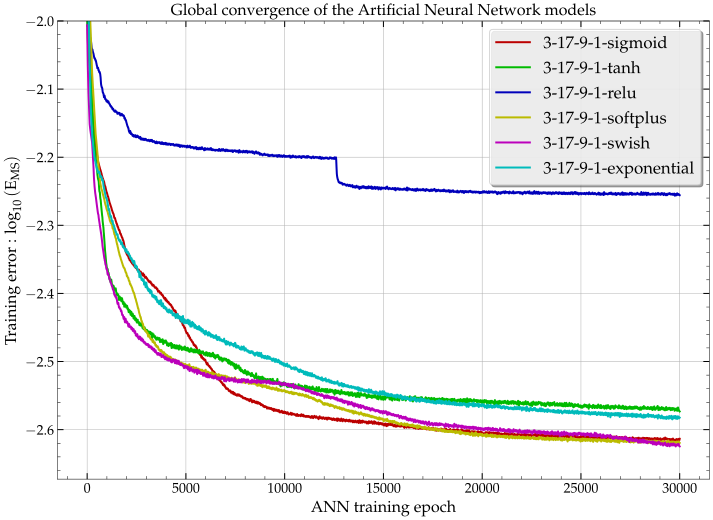
\includegraphics[width=0.8\columnwidth]{Figures/3Cr2Mo-convergence-17-9}
\caption{Global convergence of the six ANN models.}
\label{fig:ANN-conv}
\end{figure}
From this figure we can compare the convergence rates of the different networks and consider that we have reached a stationary state for all the ANNs analyzed after $30~000$ iterations.
As expected, the ReLU activation function gives the worst results with a final value of~$\MSE=3.092\times10^{-5}$, mainly due to the low number of neurons and the fact that this function is a piecewise linear function and not able to efficiently approximate the nonlinear behavior of the material.
The other five activation functions enhance more or less the same behavior, and the final value of the $\MSE$ is pretty much the same for all of them, and around $\MSE=6\times10^{-6}$.

Table~\ref{tab:Training} shows the main results from the training phase of the ANNs.
\begin{table}[h]
\caption{Comparison of the models' error depending on the activation function used.\label{tab:Training}}
\begin{tabular}{lcccccc}
\toprule
Activation & CPU time & $\MSE$ & $\RMSE$ & $\Delta\RMSE$ & $\MARE$ & $\Delta\MARE$ \\
 & & $\times 10^{-6}$ & (\MPa) & & (\%) &\\ \midrule
Sigmoid & 5:14 & 5.891 & 0.427 & 1.247 & 0.952 & 1.322\\
Tanh & 5:25 & 7.234 & 0.418 & 1.223 & 0.851 & 1.181\\
ReLU & 5:14 & 30.92 & 1.171 & 3.422 & 4.575 & 6.350\\
Softplus & 5:25 & 5.791 & 0.394 & 1.151 & 1.070 & 1.485\\
Swish & 5:31 & 5.693 & 0.342 & / &0.720 & / \\
Exp & 5:18 & 6.861 & 0.420 & 1.227 & 1.302 & 1.808\\
\bottomrule
\end{tabular}
\end{table}
We can see from this later that all models need more or less the same training time to complete the requested number of iterations.
We can see that the complexity of the activation functions has an influence on the training time, since it is greater for the Swish and Softplus functions than for the ReLU one.
We also reported in this table the real values of the~$\RMSE$ and~$\MARE$ concerning the flow stress~$\sigma$.
From this later we can see that the~$\RMSE$ is about~$0.3$ to~$0.4~\MPa$ for all activation functions except the ReLU one where the value is above~$1.1~\MPa$.
Concerning the $\MARE$, the value of all models is around~$1\%$ while it is more than~$6\%$ for the ReLU function.
Of the six activation functions used in this study, the Swish function gives the best results in terms of solution quality, while the ReLU function gives the worst.
From another point of view, the Swish activation function requires the most training time, but the difference is not discriminatory given the performance at this stage of the study.

Figure~\ref{fig:ANNFit} shows a comparison of the experimental flow stress measures during the Gleeble compression tests (reported as dots in Figure) and the predicted flow stress~$\sigma$ using the ANN for the strain rate~$\mdot{\varepsilon}=1~\ps$.
\begin{figure}[h]
\centering
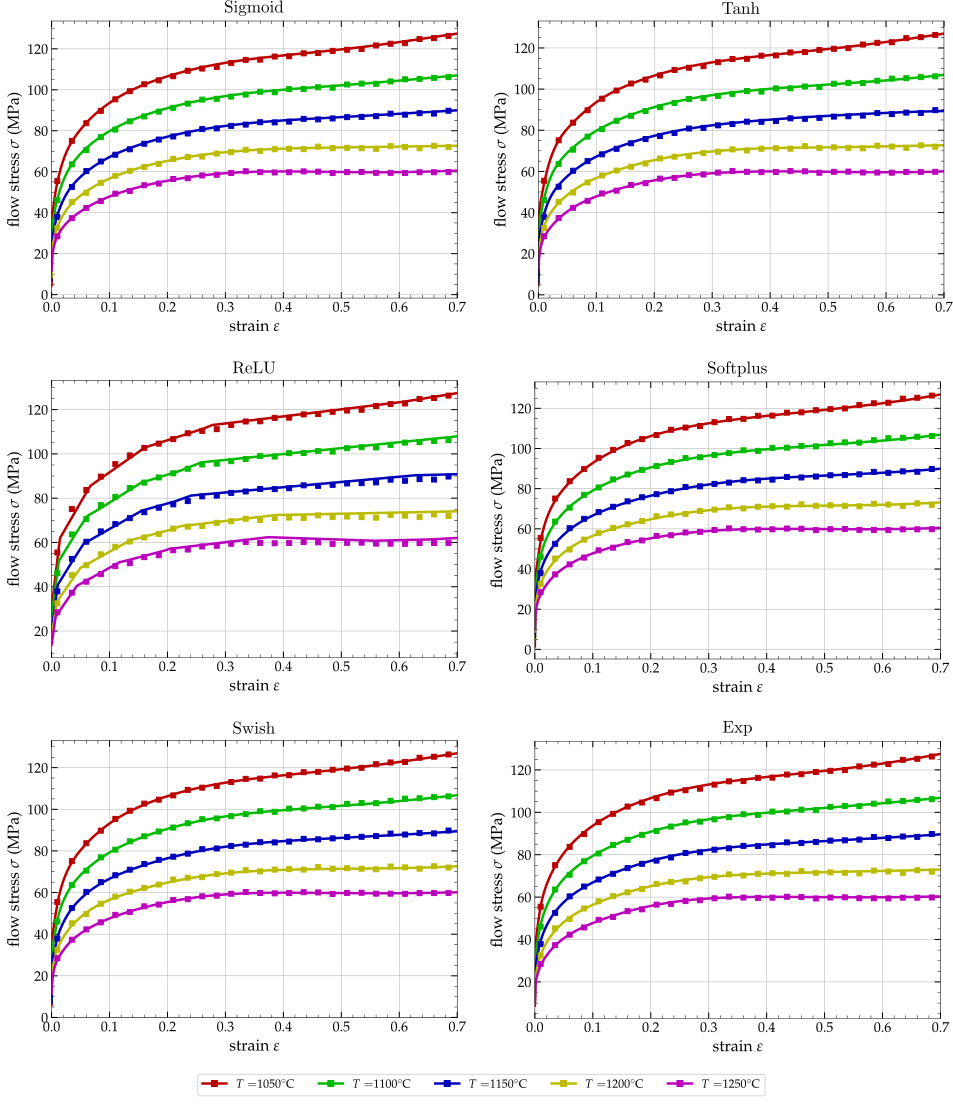
\includegraphics[width=0.95\columnwidth]{Figures/ANN-fit}
\caption{Comparison of experimental (dots) and the flow stress~$\sigma$ predicted by the ANN (continuous line) for~$\mdot{\varepsilon}=1~\ps$.}
\label{fig:ANNFit}
\end{figure}
From this later, we can see that all ANNs models are able to reproduce quite well the experimental results.
The exception is concerning the ReLU activation function where it can be seen from the results in Figure \ref{fig:ANNFit} that the predicted flow stress enhances a piecewise linear behavior.

Among the six activation functions proposed, as already presented in Section \ref{subsubsec:ANN-act}, the exponential activation function is interesting since the computation of the function and its derivative in the same step requires only one evaluation of the exponential function because $f'(x)=f(x)$ as reported in Equation (\ref{eq:act-exp}).
If we analyze the results reported in Table~\ref{tab:Training} and Figure~\ref{fig:ANNFit} concerning the exponential activation function, we can see that this one has a $\RMSE=0.420~\MPa$, $\MARE=1.302\%$ and the global behavior of the flow stress for~$\mdot{\varepsilon}=1~\ps$ is similar to the Sigmoid, Tanh, Swish or Softplus functions even if the results in terms of performance are a little below those of the other four functions.

In terms of global performance of the 3-17-9-1-exp ANN, Figure~\ref{fig:ANN-ExpFit} shows the comparison of the experimental data (dots) and the ANN flow stress for all strain rates and all temperatures defined in Section \ref{subsec:ExpTests}.
\begin{figure}[h]
\centering
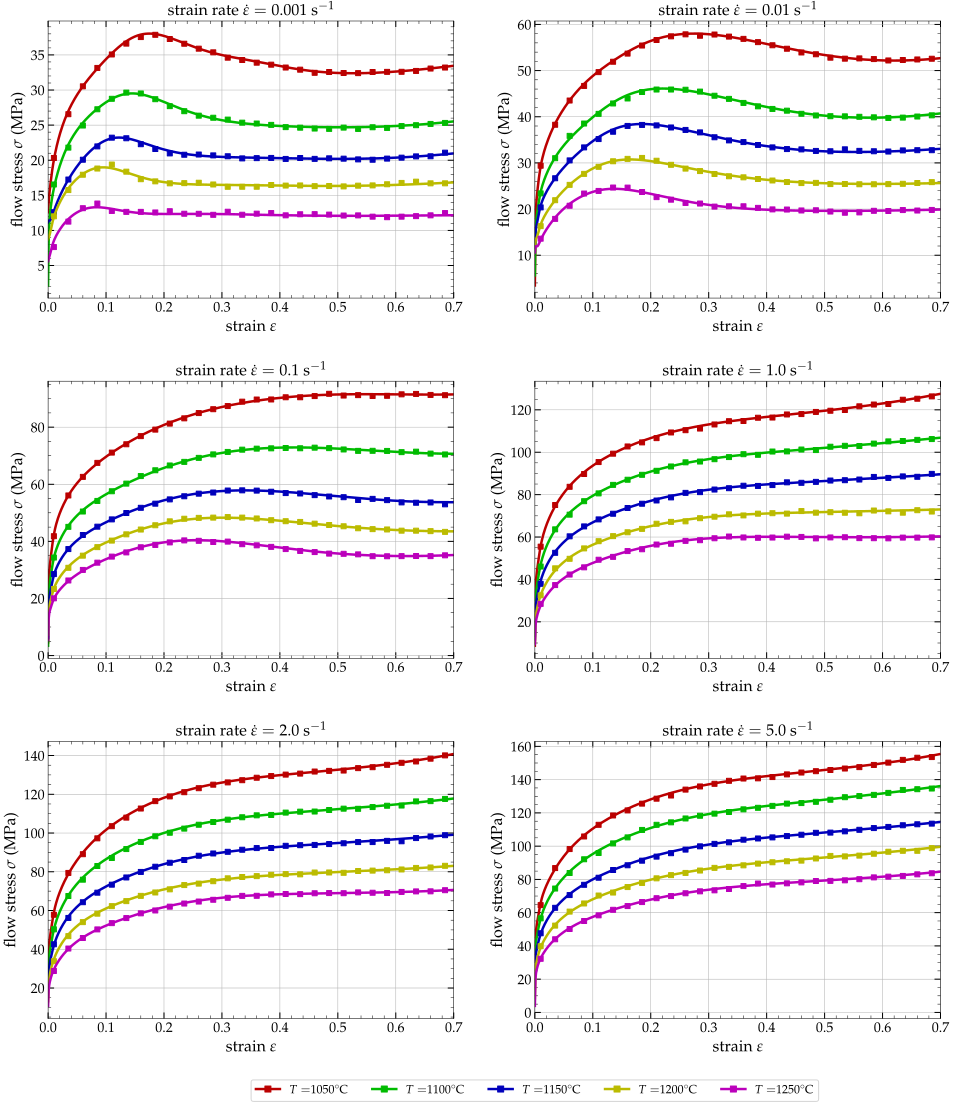
\includegraphics[width=0.95\columnwidth]{Figures/3Cr2Mo-3-17-9-1-exponential}
\caption{Comparison of experimental (dots) and the flow stress~$\sigma$ predicted by the ANN (continuous line) using the Exponential activation function.}
\label{fig:ANN-ExpFit}
\end{figure}
We can see that over the whole range of temperatures~$T$ and strain rates~$\mdot{\varepsilon}$, the performance of the model based on an exponential function is very good overall.
This model will therefore be retained for the remainder of the comparative study.

%----------------------------------------------------------------------------------
\section{Numerical simulations using the ANN flow law}\label{sec:Numerical}
%----------------------------------------------------------------------------------
Now that the flow stress models have been defined, trained and the results analyzed in terms of their relative performance in reproducing the experimental behavior recorded during compression tests on Gleeble, we will now numerically implement these models in the Abaqus FE code in the form of user routines in Fortran in order to perform numerical simulations.
After training phase, all optimized internal parameters of the ANN are stored in HDF5~\cite{Koranne-2011-HDF} files which are read by a Python program in charge to write the Fortran 77 subroutine for the Abaqus FE code.
Implementation of the flow law in the Abaqus FE code can be done using either a VUMAT (we will use the Explicit version of the Abaqus code for simulating our examples), where one have to program the computation of the stress tensor $\Sig_1$ at the end of the increment from the value of the stress tensor at the beginning of the increment $\Sig_0$ and the increment of strain $\Delta\Eps$.
This is usually done using a predictor/corrector algorithm based for example on the radial--return integration scheme~\cite{Ponthot-2002-USU}, and the curious reader can refer for example to Ming \eal~\cite{Ming-2018-ERV} for the details concerning this implementation using the Safe--Newton integration scheme or Liang \eal~\cite{Liang-2022} for a dedicated application concerning the Arrhenius flow law.
During the corrector phase, one have to evaluate the flow stress~$\sigma$ of the material as a function of the strain~$\varepsilon$, the strain rate~$\mdot{\varepsilon}$ and the temperature~$T$ at the current integration point of the element, and to solve a non-linear equation defining the plastic corrector expression and involving the computation of the three derivatives of the flow stress ~$\partial\sigma/\partial\varepsilon$, $\partial\sigma/\partial\mdot{\varepsilon}$ and~$\partial\sigma/\partial T$.
The computation of those four quantities is usually done in a subroutine called VUHARD for the Abaqus explicit FE code.
This is the function we have to implement depending on the structure and the activation functions of the ANN flow law.

\subsection{Numerical implementation of the ANN flow law}\label{subsec:Num-impl}

In order to have a better understanding of the implementation of the VUHARD subroutine, we are going to detail the procedure used to compute the flow stress and the three derivatives in one step as a function of the triplet of input values~$\varepsilon$, $\mdot{\varepsilon}$, $T$.
We suppose that the current input is stored in a three components vector $\overrightarrow{\xi}^T=\left[\varepsilon, \log(\mdot{\varepsilon}/\mdot{\varepsilon}_0), T\right]$.
We also suppose that the minimum and range values of the inputs, used during the learning phase, are stored in two vectors $\overrightarrow{\xi}_{0}$ and $\Delta\overrightarrow{\xi}$ respectively.
% The minimum and ran values of the stress are also stored in two variables $\sigma_{0}$ and $\sigma_{max}$ respectively.
\begin{itemize}
\item We first use Equation (\ref{eq:ANN-input}) to compute the vector $\overrightarrow{x}$ where all components of $\overrightarrow{\xi}$ will be remapped within the range $[0,1]$:
\begin{equation}
\overrightarrow{x}=\left(\overrightarrow{\xi}-\overrightarrow{\xi}_{0}\right)\oslash\Delta\overrightarrow{\xi},
\end{equation}
where $\oslash$ is the Hadamard division operator.
\item Conforming to Equation (\ref{eq:ANN-y}), we compute the vector:
\begin{equation}
\overrightarrow{y}\lay{1}=\w\lay{1}\cdot\overrightarrow{x}+\overrightarrow{b}\lay{1}.
\end{equation}
\item Then, from Equation (\ref{eq:ANN-f}) and the expression of the activation function used for the first layer of the ANN and defined by one of the Equations (\ref{eq:act-sig}-\ref{eq:act-exp}), we compute the vector:
\begin{equation}
\overrightarrow{\hat{y}}\lay{1}=f\lay{1}(\overrightarrow{y}\lay{1}).
\end{equation}
\item We repeat the process for the second layer, so that we compute the vectors: \begin{equation}
\overrightarrow{y}\lay{2}=\w\lay{2}\cdot\overrightarrow{\hat{y}}\lay{1}+\overrightarrow{b}\lay{2},
\end{equation}
and:
\begin{equation}
\overrightarrow{\hat{y}}\lay{2}=f\lay{2}(\overrightarrow{y}\lay{2}).
\end{equation}
\item From Equations (\ref{eq:ANN-s}) and (\ref{eq:ANN-output}), we compute the flow stress $\sigma$ using the following equation:
\begin{equation}
s = \Delta\sigma.\left(\overrightarrow{w}^T \dotp \overrightarrow{\hat{y}}\lay{2} + b\right) + \sigma_{0}.
\end{equation}
\item Then we can compute in a single step the three derivatives $\overrightarrow{\sigma}'$ from Equation (\ref{eq:ANN-der}) with the following expression:
\begin{equation}
\begin{array}{l}
\overrightarrow{\Sig}' = \Delta\sigma.\w\lay{1}^T \dotp\left[\left(\w\lay{2}^T \dotp \left(\overrightarrow{w}^T \circ f'(\overrightarrow{y}\lay{2})\right)\right) \circ f'(\overrightarrow{y}\lay{1})\right] \oslash \Delta\overrightarrow{\xi}\\
\Sig_2' := \Sig_2' / \mdot{\varepsilon}
\end{array},
\end{equation}
where the expression used for $f'()$ changes depending on the activation function used.
\end{itemize}
As an illustration the corresponding implementation using Python of those equations is proposed in Figure~\ref{fig:PythonStress}, where the arguments of the functions are \var{xi} for the $\overrightarrow{\xi}$ vector, \var{deps} for $\mdot{\varepsilon}$, \var{Act} for the activation function and \var{dAct} for the derivative of the activation function.
The network architecture is defined by the numpy arrays \var{w1}, \var{w2}, \var{w}, \var{b1}, \var{b2} and \var{b}.
The other variables \var{xi0}, \var{Dxi}, \var{sig0} and \var{Dsig} correspond to the quantities $\overrightarrow{\xi}_{0}$, $\Delta\overrightarrow{\xi}$, $\sigma_{0}$ and $\Delta\sigma$ respectively.
\begin{figure}[h]
\begin{PythonListing}
def stressAndDerivatives(xi, deps, Act, dAct):
  x = (xi - xi0) / Dxi
  y1 = w1.dot(x) + b1
  yh1 = Act(y1)
  y2 = w2.dot(yh1) + b2
  yh2 = Act(y2)
  Sig = Dsig*(w.dot(yh2) + b) + sig0
  dSig = Dsig*((w1.T).dot((w2.T).dot(w.T*dAct(y2))*dAct(y1))) / Dxi
  dSig[1] = dSig[1] / deps
  return Sig, dSig
\end{PythonListing}
\caption{Python function to compute the flow stress and the derivative vector.\label{fig:PythonStress}}
\end{figure}

A Python program is used to analyze the code reported in Figure~\ref{fig:PythonStress} and translate it into a Fortran 77 subroutine.
During the translation phase, all functions corresponding to array operators, as matrix--matrix multiplications or element-wise operations, are converted into unrolled loops (explicitly written), all values of the ANNs parameters are explicitly written as data at the beginning of the subroutine, so that the a 3-17-9-1-exp Fortran routine consist of more than 400 lines of code.
A small extract of the corresponding VUHARD subroutine is presented in Figure \ref{fig:FortranStress}.
\begin{figure}[h]
\begin{FortranListing}
      subroutine vuhard (... Heading of VUHARD routine ...)
      ...
c Block of Data
      double precision w1(17, 3)
      data w1/-18.005151041D0, -2.1260391826D0, -2.150871965D0,
     + -0.8321546516D0,...
      ...
c Preprocessing of the variables
      xeps = (eqps(k) - xmI(1))/xrI(1)
      xdeps = (log(eqpsRate(k)/xdeps0) - xmI(2))/xrI(2)
      xtemp = (tempNew(k) - xmI(3))/xrI(3)
c Hidden layer #1 (y10 to y116)
      y10 = w1(1,1)*xeps + w1(1,2)*xdeps + w1(1,3)*xtemp + b1(1)
      ...
c exponential activation function (yh10 to yh116)
      yh10 = exp(y10)
      ...
c Hidden layer #2 (y20 to y28)
      y20 = w2(1,1)*yh10 + w2(1,2)*yh11 + w2(1,3)*yh12
     + +w2(1,4)*yh13 + ... + b2(1)
      ...
c exponential activation function (yh20 to yh28)
      yh20 = exp(y20)
      ...
c Derivatives terms (xa0 to xa8), (xb0 to xb16)
      xa0 = w3(1)*yh20
      ...
      xb0 = (w2(1,1)*xa0 + w2(2,1)*xa1 + w2(3,1)*xa2
     + +w2(4,1)*xa3 + ... + w2(9,1)*xa8)*yh10
      ...
c Outputs of the subroutine
      Yield(k) = xrO*(w3(1)*yh20 + w3(2)*yh21
     + +w3(3)*yh22 + ... +b3) + xmO
      dyieldDeqps(k,1) = xrO*(w1(1,1)*xb0 + w1(2,1)*xb1
     + +w1(3,1)*xb2 + ... + w1(17,1)*xb16) / xrI(1)
      dyieldDeqps(k,2) = xrO*(w1(1,2)*xb0 + w1(2,2)*xb1
     + +w1(3,2)*xb2 + ... + w1(17,2)*xb16)/(xrI(2)*eqpsRate(k))
      dyieldDtemp(k) = xrO*(w1(1,3)*xb0 + w1(2,3)*xb1
     + +w1(3,3)*xb2 + ... + w1(17,3)*xb16) / xrI(3)
c Return from the VUHARD subroutine
      return
      end
\end{FortranListing}
\caption{Part of the VUHARD Fortran 77 subroutine for the ANN flow law and the exponential activation function.\label{fig:FortranStress}}
\end{figure}
Depending on the kind of activation function used, some lines differ from one version to the other one, such as the definitions of the activation functions (see line 16 in Figure~\ref{fig:FortranStress}) and the expressions of the internal variables \var{xa} and \var{xb} (see lines 26 and 28 in Figure~\ref{fig:FortranStress}). Figure~\ref{fig:FortranSigmoid} show the declaration of the Sigmoid activation function and its derivative, while Figure~\ref{fig:FortranSoftplus} show the same part of the code with the use of the Softplus activation function.
\begin{figure}[h]
\begin{FortranListing}
c sigmoid activation function (yh10 to yh116)
      yh10 = 1/(1 + exp(-y10))
      ...
c Derivatives terms (xa0 to xa8), (xb0 to xb16)
      xa0 = w3(1)*(yh20*(1 - yh20))
      ...
      xb0 = (w2(1,1)*xa0 + w2(2,1)*xa1 + w2(3,1)*xa2
     + +w2(4,1)*xa3 + ... + w2(9,1)*xa8)*(yh10*(1 - yh10))
      ...
\end{FortranListing}
\caption{Part of the VUHARD Fortran 77 subroutine with the Sigmoid activation function.\label{fig:FortranSigmoid}}
\end{figure}
\begin{figure}[h]
\begin{FortranListing}
c softplus activation function (yh10 to yh116)
      yh10 = log(1 + exp(y10))
      ...
c Derivatives terms (xa0 to xa8), (xb0 to xb16)
      xa0 = w3(1)*(1/(1 + exp(-y20)))
      ...
      xb0 = (w2(1,1)*xa0 + w2(2,1)*xa1 + w2(3,1)*xa2
     + +w2(4,1)*xa3 + ... + w2(9,1)*xa8)*(1/(1 + exp(-y10)))
      ...
\end{FortranListing}
\caption{Part of the VUHARD Fortran 77 subroutine with the Softplus activation function.\label{fig:FortranSoftplus}}
\end{figure}


The Fortran subroutine is compiled with double precision directive using the Intel Fortran 14.0.2 compiler on a Ubuntu 22.04 server and linked to the main Abaqus explicit executable.

\subsection{Numerical simulations and comparisons}\label{subsec:Num-sim}

To compare the influence of choosing different type of activation functions on the numerical results using the Abaqus explicit software, we have made the choice to simulate the compression test presented in Section \ref{subsec:ExpTests}.
We consider therefore a medium-carbon steel, type P20 cylinder in compression with an initial diameter of~$d=10$~mm and a height of~$h_0=15$~mm as reported in Figure~\ref{fig:Num-model}.
\begin{figure}[h]
\centering
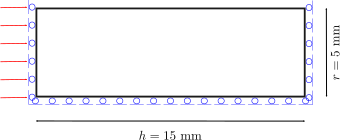
\includegraphics[width=0.65\columnwidth]{Figures/CyCompression}
\caption{Axis-symmetric model for the numerical simulation of the compression of a cylinder.}
\label{fig:Num-model}
\end{figure}
At the end of the compression process, the final height of the cylinder is~$h_f=6$~mm, so that the reduction is $60\%$. 
The displacement is applied with a constant speed and the simulation time is fixed to $t=1$~s, so that the strain rate is around $1~\ps$ during the simulation at the center of the specimen.
%The six ANN flow laws will be compared here-after.
The mesh consists of $850$ axis-symmetric quadrilateral finite elements with 4 nodes and reduced integration (CAX4R) with 50 elements along the axis direction and 17 elements along the radial direction.
The cylinder is between two rigid surfaces and a Coulomb friction law with a friction coefficient $\mu=0.15$ is used.
A global mass scaling with a value of $M_s=1000$ is used to reduce the computing time by a factor of $31.6$.
The initial temperature of the material is set to $T_0=1050\celsius$ and we use an explicit adiabatic solver for the simulation of the compression process. 
%The elastic properties of the material are fixed to a Young modulus $E=207~\GPa$ and a Poisson ration $\nu=0.285$.

The average strain rate during the compression for the center element of the specimen is around~$\mdot{\overline{\varepsilon}^p}=0.8~\ps$.

\begin{table}[h]
\caption{Table}
\begin{tabular}{lcccccc}
\toprule
Activation & CPU time & $N_{inc}$ & $N_{inc}$/s & $\overline{\varepsilon}^p$ & $\overline{\sigma}$ & $T$\\
 & (s) & & & & (\MPa) &(\celsius)\\ \midrule
Sigmoid & 1089 & 1~251~869 & 1150 & 0.787 & 126.8 & 1071.1 \\
Tanh & 1202 & 1~253~740 & 1043 & 0.786 & 125.2 & 1070.6 \\
ReLU & 915 & 1~247~899 & 1364 & 0.787 & 128.4 & 1071.1 \\
Softplus & 1795 & 1~245~146 & 694 & 0.783 & 125.2 & 1070.2 \\
Swish & 1322 & 1~246~006 & 943 & 0.789 & 123.7 & 1071.0 \\
Exp & 998 & 1~250~145 & 1253 & 0.787 &122.5 &1070.5 \\
\bottomrule
\end{tabular}
\end{table}

\begin{figure}[h]
\centering
\includegraphics[width=0.8\columnwidth]{Figures/MisesHalf}
\caption{xx.}
\label{fig:Num-misesCP}
\end{figure}

\begin{figure}[h]
\centering
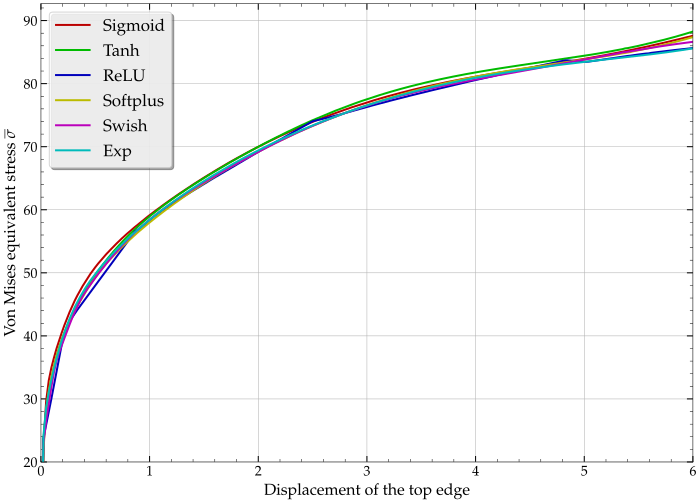
\includegraphics[width=0.8\columnwidth]{Figures/vonMises}
\caption{xx.}
\label{fig:Num-misesTH}
\end{figure}
%----------------------------------------------------------------------------------
\section{Conclusions and future work}\label{sec:Conclusions}
%----------------------------------------------------------------------------------

%%%%%%%%%%%%%%%%%%%%%%%%%%%%%%%%%%%%%%%%%%
%\section{Patents}


%%%%%%%%%%%%%%%%%%%%%%%%%%%%%%%%%%%%%%%%%%
\vspace{6pt}

%%%%%%%%%%%%%%%%%%%%%%%%%%%%%%%%%%%%%%%%%%
%% optional
%\supplementary{The following supporting information can be downloaded at: \linksupplementary{s1}, Figure S1: title; Table S1: title; Video S1: title.}

% Only for the journal Methods and Protocols:
% If you wish to submit a video article, please do so with any other supplementary material.
% \supplementary{The following supporting information can be downloaded at: \linksupplementary{s1}, Figure S1: title; Table S1: title; Video S1: title. A supporting video article is available at doi: link.}

%%%%%%%%%%%%%%%%%%%%%%%%%%%%%%%%%%%%%%%%%%
%\authorcontributions{
%Conceptualization, P.T.M. and O.P.;
%methodology, O.P.;
%software, P.T.M. and O.P.;
%validation, O.P.;
%formal analysis, O.P.;
%investigation, P.D.;
%resources, P.D. and M.J.;
%data curation, P.T.M. and P.D.;
%writing---original draft preparation, P.T.M.;
%writing---review and editing, O.P.;
%visualization, O.P.;
%supervision, M.J., A.T. and O.P.;
%project administration, M.J.;
%funding acquisition, M.J.
%All authors have read and agreed to the published version of the manuscript.}

\funding{This research received no external funding.}

%\institutionalreview{In this section, you should add the Institutional Review Board Statement and approval number, if relevant to your study. You might choose to exclude this statement if the study did not require ethical approval. Please note that the Editorial Office might ask you for further information. Please add “The study was conducted in accordance with the Declaration of Helsinki, and approved by the Institutional Review Board (or Ethics Committee) of NAME OF INSTITUTE (protocol code XXX and date of approval).” for studies involving humans. OR “The animal study protocol was approved by the Institutional Review Board (or Ethics Committee) of NAME OF INSTITUTE (protocol code XXX and date of approval).” for studies involving animals. OR “Ethical review and approval were waived for this study due to REASON (please provide a detailed justification).” OR “Not applicable” for studies not involving humans or animals.}

%\informedconsent{Any research article describing a study involving humans should contain this statement. Please add ``Informed consent was obtained from all subjects involved in the study.'' OR ``Patient consent was waived due to REASON (please provide a detailed justification).'' OR ``Not applicable'' for studies not involving humans. You might also choose to exclude this statement if the study did not involve humans.
%
%Written informed consent for publication must be obtained from participating patients who can be identified (including by the patients themselves). Please state ``Written informed consent has been obtained from the patient(s) to publish this paper'' if applicable.}

\dataavailability{Source files of the numerical simulations are available from the author.}

%\acknowledgments{In this section you can acknowledge any support given which is not covered by the author contribution or funding sections. This may include administrative and technical support, or donations in kind (e.g., materials used for experiments).}

\conflictsofinterest{The author declare no conflict of interest.}

%%%%%%%%%%%%%%%%%%%%%%%%%%%%%%%%%%%%%%%%%%
%% Optional
%\sampleavailability{Samples of the compounds ... are available from the authors.}

%% Only for journal Encyclopedia
%\entrylink{The Link to this entry published on the encyclopedia platform.}

\abbreviations{Abbreviations}{
The following abbreviations are used in this manuscript:\\

\noindent
\begin{tabular}{@{}ll}
ANN & Artificial neural network \\
%AR & Arrhenius \\
CPU & Central processing unit \\
%DRV & Dynamic recovery\\
%DRX & Dynamic recrystallization \\
FE & Finite Element \\
%HS & Hansel--Spittel \\
%JC & Johnson--Cook \\
%MZA & Modified-Zerilli--Armstrong \\
%WH & Work hardening \\
%ZA & Zerilli--Armstrong
\end{tabular}
}

%%%%%%%%%%%%%%%%%%%%%%%%%%%%%%%%%%%%%%%%%%
%% Optional
\appendixtitles{no} % Leave argument "no" if all appendix headings stay EMPTY (then no dot is printed after "Appendix A"). If the appendix sections contain a heading then change the argument to "yes".
%\appendixstart
%\appendix
%%----------------------------------------------------------------------------------
%\section[\appendixname~\thesection]{ANN Flow Law Coefficients\label{sec:Appendix}}
%%----------------------------------------------------------------------------------
%
%In order to complete this paper, we report here after the computing process and the $240$~coefficients of the artificial neural network ANN-3-17-9-1-exp model.
%The weight matrix for the first hidden layer $\w_1$ is a $17\times3$ matrix:
%\begin{equation*}
%\w_1 = \left[
%\begin{array}{rrr}
%-18.005 & 1.250 & -1.342\\
%-2.126 & 0.829 & -4.838\\
%-2.151 & 4.882 & -1.110\\
%-0.832 & -4.702 & 0.888\\
%1.348 & 1.259 & -1.429\\
%-0.397 & 2.798 & 0.710\\
%-8.646 & -5.529 & -3.916\\
%0.835 & 3.751 & -37.522\\
%0.362 & 0.118 & 8.211\\
%-6.782 & 1.091 & 0.319\\
%-0.386 & 0.794 & -1.934\\
%-0.030 & -4.024 & 0.773\\
%1.488 & -2.371 & 4.147\\
%-10.993 & -8.295 & -12.164\\
%-2.439 & -0.757 & -0.323\\
%-280.787 & 1.176 & -0.090\\
%-3.538 & -2.779 & -19.796\\
%\end{array}\right]
%\end{equation*}
%
%The biases of the first hidden layer $\overrightarrow{b_1}$ is a $17$-component vector:
%\begin{equation*}
%\overrightarrow{b}_1 = \left[
%\begin{array}{r}
%-0.610\\
%-2.237\\
%-4.040\\
%1.134\\
%-3.054\\
%-3.478\\
%1.501\\
%-5.838\\
%-8.602\\
%-1.245\\
%-1.556\\
%0.738\\
%-5.335\\
%2.208\\
%-0.629\\
%-1.619\\
%-0.080\\
%\end{array}\right]
%\end{equation*}
%
%The weight matrix for the second hidden layer $\w_2$ is a $9\times17$ matrix:
%\begin{equation*}
%\w_2^T = \left[
%\begin{array}{rrrrrrrrr}
%0.133 & -86.946 & -1.051 & 1.803 & -1.850 & -0.440 & -7.127 & 0.174 & -0.340\\
%7.083 & -20.359 & 4.734 & 2.643 & 1.095 & -0.023 & -27.715 & -0.822 & -0.648\\
%-4.270 & -42.833 & -1.828 & -0.537 & 0.706 & 0.311 & -52.811 & 0.850 & -0.099\\
%-4.290 & 2.243 & -30.375 & 0.054 & 1.164 & -1.643 & -1.862 & 0.987 & -1.024\\
%-9.379 & -2.773 & 0.583 & -3.396 & -7.241 & -1.776 & -13.472 & 0.536 & -2.769\\
%-8.435 & -8.215 & 1.744 & 0.019 & 2.242 & 0.089 & -15.298 & -2.382 & -6.080\\
%8.050 & -3.032 & -10.094 & 0.164 & -3.551 & -0.090 & 4.431 & -1.937 & 3.075\\
%-33.193 & -1.846 & -2.293 & -2.618 & 16.397 & -1.025 & -2.828 & 1.294 & 6.319\\
%2.114 & 1.389 & -0.987 & -0.090 & -1.819 & -0.097 & 2.508 & 0.687 & 0.878\\
%-2.214 & -14.317 & -2.055 & 0.387 & 1.097 & -0.712 & 8.227 & -3.942 & -1.930\\
%-13.351 & 1.743 & 3.924 & -5.355 & -6.500 & 1.088 & 3.149 & -1.526 & -0.613\\
%-2.844 & -3.412 & -11.884 & 0.033 & -2.475 & -1.387 & 2.261 & -1.787 & -0.300\\
%-13.599 & -5.833 & 8.660 & 0.092 & -4.317 & 1.483 & -14.671 & -5.869 & 1.144\\
%-23.598 & 0.261 & 18.128 & -0.031 & -2.716 & -0.374 & -72.263 & 0.565 & -1.063\\
%2.988 & -3.510 & 5.437 & -1.166 & -7.761 & 2.746 & 3.329 & -2.348 & -0.459\\
%-0.526 & -14.870 & 6.458 & 0.036 & 8.939 & -0.659 & -12.182 & -37.338 & 13.056\\
%11.909 & 4.178 & -9.257 & -0.170 & 6.748 & 0.415 & 3.328 & 1.992 & -1.880\\
%\end{array}\right]
%\end{equation*}
%
%The biases of the second hidden layer $\overrightarrow{b_2}$ are a $9$-component vector:
%\begin{equation*}
%\overrightarrow{b}_2 = \left[
%\begin{array}{r}
%1.870\\
%-0.240\\
%-2.207\\
%-2.724\\
%-6.895\\
%-2.259\\
%-4.667\\
%-1.252\\
%-5.038\\
%\end{array}\right]
%\end{equation*}
%
%The weight vector for the output layer $\overrightarrow{w}$ is a $9$-component vector:
%\begin{equation*}
%\overrightarrow{w} = \left[
%\begin{array}{r}
%-4.128\\
%-3.015\\
%1.521\\
%-2.322\\
%-1.324\\
%1.633\\
%-3.175\\
%2.454\\
%-3.135\\
%\end{array}\right]
%\end{equation*}
%
%The bias of the output layer $b$ is a scalar:
%\begin{equation*}
%b = 0.242
%\end{equation*}

%The boundaries of the range of the corresponding field~are as follows:
%\begin{itemize}
%\item $\varepsilon^p\!\in\!\left[0.0,0.7\right]$
%\item $\mdot{\varepsilon}\!\in\!\left[0.001~\ps,0.1~\ps\right]$
%\item $T\!\in\!\left[750~\celsius,1300~\celsius\right]$
%\item $\sigma\!\in\!\left[3.052~\MPa,306.096~\MPa\right]$.
%\end{itemize}
%
%The reference strain rate is $\mdot{\varepsilon_0} = 0.001~\ps$.

%%%%%%%%%%%%%%%%%%%%%%%%%%%%%%%%%%%%%%%%%%
\begin{adjustwidth}{-\extralength}{0cm}
%\printendnotes[custom] % Un-comment to print a list of endnotes

\reftitle{References}

% Please provide either the correct journal abbreviation (e.g. according to the “List of Title Word Abbreviations” http://www.issn.org/services/online-services/access-to-the-ltwa/) or the full name of the journal.
% Citations and References in Supplementary files are permitted provided that they also appear in the reference list here.

%=====================================
% References, variant A: external bibliography
%=====================================
\bibliography{bibliography}

% If authors have biography, please use the format below
%\section*{Short Biography of Authors}
%\bio
%{\raisebox{-0.35cm}{\includegraphics[width=3.5cm,height=5.3cm,clip,keepaspectratio]{Definitions/author1.pdf}}}
%{\textbf{Firstname Lastname} Biography of first author}
%
%\bio
%{\raisebox{-0.35cm}{\includegraphics[width=3.5cm,height=5.3cm,clip,keepaspectratio]{Definitions/author2.jpg}}}
%{\textbf{Firstname Lastname} Biography of second author}

% For the MDPI journals use author-date citation, please follow the formatting guidelines on http://www.mdpi.com/authors/references
% To cite two works by the same author:~\citeauthor{ref-journal-1a} (\citeyear{ref-journal-1a},~\citeyear{ref-journal-1b}). This produces: Whittaker (1967, 1975)
% To cite two works by the same author with specific pages:~\citeauthor{ref-journal-3a} (\citeyear{ref-journal-3a}, p. 328;~\citeyear{ref-journal-3b}, p.475). This produces: Wong (1999, p. 328; 2000, p. 475)

%%%%%%%%%%%%%%%%%%%%%%%%%%%%%%%%%%%%%%%%%%
%% for journal Sci
%\reviewreports{\\
%Reviewer 1 comments and authors’ response\\
%Reviewer 2 comments and authors’ response\\
%Reviewer 3 comments and authors’ response
%}
%%%%%%%%%%%%%%%%%%%%%%%%%%%%%%%%%%%%%%%%%%
\PublishersNote{}
\end{adjustwidth}
\end{document}

